\documentclass[border=1cm]{standalone}
\usepackage{tikz}
\usepackage{pgfplots}
\pgfplotsset{compat=1.12}

\usetikzlibrary{calc}
\usetikzlibrary{shapes.multipart}
\usetikzlibrary{positioning}

\tikzstyle{edge} = [draw, thick, shorten >=2pt, shorten <=2pt]
\tikzstyle{directed} = [edge, arrows={-latex}, shorten >=2pt, shorten <=0pt]
\tikzstyle{marked} = [tumred]
\tikzstyle{marked edge} = [very thick, marked]
\tikzstyle{marked node} = [very thick, draw=tumred, fill=tumred!15]
\tikzstyle{every text node part} = [align=center, execute at begin node=\setlength{\baselineskip}{2ex}]

%%%%%%%%%%%%
%  Locale  %
%%%%%%%%%%%%
\usepackage[english]{babel}
\selectlanguage{english}
\usepackage[T1]{fontenc}
\usepackage[utf8]{inputenc}

%%%%%%%%%%%
%  Fonts  %
%%%%%%%%%%%
\usepackage{textcomp}
\usepackage[sc,osf]{mathpazo}
% For scales see http://tex.stackexchange.com/a/2506
\usepackage[scaled=0.86]{berasans}
\usepackage[scaled=1.03]{inconsolata}
\linespread{1.05}
\usepackage{microtype}

%%%%%%%%%%%
%  Stuff  %
%%%%%%%%%%%
\usepackage{amsmath}

%%%%%%%%%%%%
%  Colors  %
%%%%%%%%%%%%
% Base Colors Corporate Design
\definecolor{tumblue}{HTML}{0065BD}
\definecolor{tumgreen}{HTML}{A2AD00}
\definecolor{tumorange}{HTML}{E37222}
\definecolor{tumivory}{HTML}{DAD7CB}
\definecolor{tumred}{HTML}{E53418} % not in Styleguide

% Derived Colors
% https://kuler.adobe.com/create/color-wheel/
% https://portal.mytum.de/corporatedesign/print/styleguide/
% Grays - TUM
\definecolor{tumgray0}{HTML}{000000}
\definecolor{tumgray1}{HTML}{58585A}
\definecolor{tumgray2}{HTML}{9C9D9F}
\definecolor{tumgray3}{HTML}{D9DADB}
\definecolor{tumgray4}{HTML}{FFFFFF}

% Blues - TUM
\definecolor{tumblue0}{HTML}{003359}
\definecolor{tumblue1}{HTML}{005293}
\definecolor{tumblue2}{HTML}{0073CF}
\definecolor{tumblue3}{HTML}{64A0C8}
\definecolor{tumblue4}{HTML}{98C6EA}

% Greens - Adobe
\definecolor{tumgreen0}{HTML}{EAF900}
\definecolor{tumgreen1}{HTML}{AEBA00}
\definecolor{tumgreen2}{HTML}{8A9300}
\definecolor{tumgreen3}{HTML}{525800}

% Reds - Adobe
\definecolor{tumred0}{HTML}{F23719}
\definecolor{tumred1}{HTML}{CB2E15}
\definecolor{tumred2}{HTML}{90210F}
\definecolor{tumred3}{HTML}{65170B}

% Oranges - Adobe
\definecolor{tumorange0}{HTML}{F07824}
\definecolor{tumorange1}{HTML}{C9651E}
\definecolor{tumorange2}{HTML}{8E4715}
\definecolor{tumorange3}{HTML}{63320F}


\begin{document}
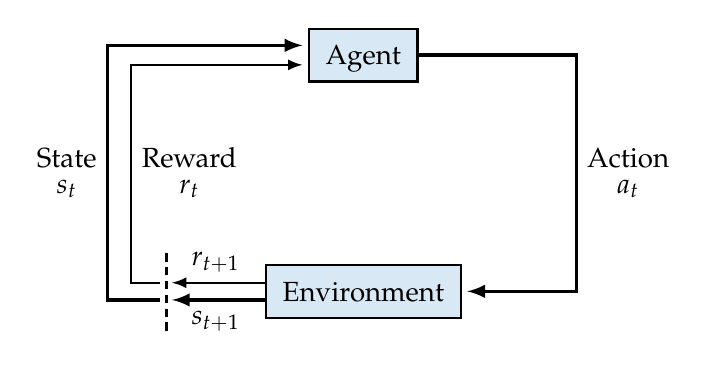
\begin{tikzpicture}
    \tikzstyle{entity} = [draw, fill=tumblue!15, thick, inner sep=6pt];

    \node[entity, text height=1.5ex, text depth=0ex] (agent) at (0, 3) {Agent};
    \node[entity, text height=1.5ex, text depth=0ex] (env) at (0, 0) {Environment};

    \draw[edge, directed, very thick] (agent.east) -- ++(2, 0) -- node[midway, right] {Action \\ $a_t$} ++(0, -3) -- (env.east);

    \draw[edge, directed, very thick] (env.185)++(-1.25, 0) -- ++(-0.75, 0) |- node[pos=0.25, left] {State \\ $s_t$} node[pos=0.25, right, shift={(0.3, 0)}] {Reward \\ $r_t$} (agent.170);
    \draw[edge, directed] (env.175)++(-1.25, 0) -- ++(-0.45, 0) |- (agent.190);

    \draw[preaction={draw, line width=5pt, white}, thick, densely dashed] (env.west) ++(-1.25, -0.5) -- ++(0, 1);
    \draw[edge, directed, very thick] (env.185) -- node[below] {$s_{t+1}$} ++(-1.25, 0);
    \draw[edge, directed] (env.175) -- node[above] {$r_{t+1}$} ++(-1.25, 0);
\end{tikzpicture}
\end{document}
